182. \begin{figure}[ht!]
\center{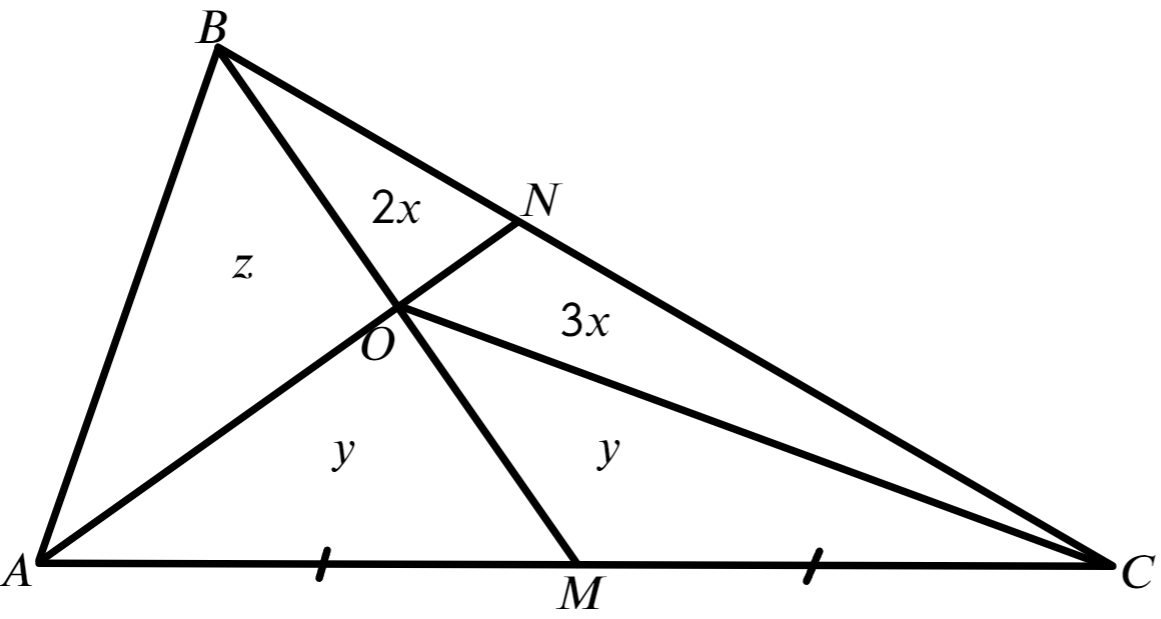
\includegraphics[scale=0.35]{g9-182.png}}
\end{figure}\\
Так как $BN:BC=0,4=\cfrac{2}{5},$ то $NC=\cfrac{3}{5}BC$ и $BN:NC=\cfrac{2}{3}.$ Площади треугольников с общей высотой относятся так же, как стороны, на которые опущена эта высота, поэтому введём обозначения $S_{\Delta BON}=2x,\ S_{\Delta NOC}=3x,\ S_{\Delta AOM}=S_{\Delta COM}=y,\ S_{\Delta AOB}=z.$ Из треугольников $ABM$ и $BMC$ получим равенство $z+y=2x+3x+y,\ z=5x.$ Из треугольников $ABN$ и $ANC$ имеем равенство $\cfrac{5x+2x}{y+y+3x}=\cfrac{2}{3},\ 21x=4y+6x,\ y=\cfrac{15}{4}x.$
Тогда $BO:OM=\cfrac{2x+3x}{\cfrac{15}{4}x}=\cfrac{4}{3}=4:3.$\\
